\documentclass[border=6pt]{standalone}
\usepackage{tikz}
\usetikzlibrary{arrows.meta,positioning,calc,decorations.pathreplacing}
\begin{document}
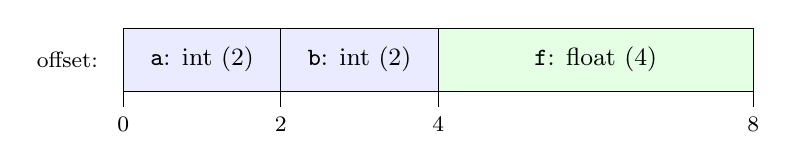
\begin{tikzpicture}[>=Stealth,font=\small,
 cell/.style={draw,minimum height=0.8cm,align=center}]
\node[cell,minimum width=2.0cm,fill=blue!8] at (1.0,0) {\texttt{a}: int (2)};
\node[cell,minimum width=2.0cm,fill=blue!8] at (3.0,0) {\texttt{b}: int (2)};
\node[cell,minimum width=4.0cm,fill=green!10] at (6.0,0) {\texttt{f}: float (4)};
\foreach \x/\l in {0/0,2/2,4/4,8/8} \draw (\x,-0.4) -- (\x,-0.6) node[below,font=\footnotesize] {\l};
\node[font=\footnotesize,anchor=east] at (-0.2,0) {offset:};
\end{tikzpicture}
\end{document}
